\documentclass[a4paper, 11pt, notitlepage, english]{article}

\usepackage{babel, textcomp}
\usepackage[utf8]{inputenc}
\usepackage[T1]{fontenc, url}
\usepackage{amsmath, amssymb}
\usepackage{amsbsy, amsfonts}
\usepackage{graphicx, color, xcolor}
\usepackage{framed, parskip, titling}
\usepackage{flafter, caption, multicol}
\usepackage{verbatim, listings}
\usepackage{shadow}
\usepackage{url}
\usepackage{framed}
\usepackage{fancyvrb}
\usepackage{titling}


%\DeclareCaptionLabelSeparator{colon}{. }
\renewcommand{\captionfont}{\sffamily}
\renewcommand{\captionlabelfont}{\bf\sffamily}
\setlength{\captionmargin}{40pt}

\setcounter{tocdepth}{2}

% \lstset{language=c++}
% \lstset{basicstyle=\footnotesize\sffamily,
%   numbers=left,                   % where to put the line-numbers
%   numberstyle=\tiny\color{gray},  % the style that is used for the line-numbers
%   stepnumber=2, }
% \lstset{backgroundcolor=\color{white}}
% \lstset{frame=single}
% \lstset{stringstyle=\sffamily}
% \lstset{keywordstyle=\color{red}\bfseries}
% \lstset{commentstyle=\color{blue}}
% \lstset{showspaces=false}
% \lstset{showstringspaces=false}
% \lstset{showtabs=false}
% \lstset{tabsize=2}
% \lstset{breaklines}

\definecolor{javared}{rgb}{0.6,0,0} % for strings
\definecolor{javagreen}{rgb}{0.25,0.5,0.35} % comments
\definecolor{javapurple}{rgb}{0.5,0,0.35} % keywords
\definecolor{javadocblue}{rgb}{0.25,0.35,0.75} % javadoc

\lstset{language=c++,
basicstyle=\ttfamily\footnotesize,
keywordstyle=\color{javapurple}\bfseries,
stringstyle=\color{javared},
commentstyle=\color{javagreen},
morecomment=[s][\color{javadocblue}]{/**}{*/},
numbers=left,
numberstyle=\tiny\color{black},
stepnumber=2,
numbersep=10pt,
tabsize=2,
showspaces=false,
showstringspaces=false,
frame= single,
breaklines=true}



\usepackage{geometry}
\geometry{headheight=0.01mm}
\geometry{top=24mm, bottom=29mm, left=39mm, right=39mm}

\renewcommand{\arraystretch}{2}
\setlength{\tabcolsep}{10pt}
% \makeatletter
% \renewcommand*\env@matrix[1][*\c@MaxMatrixCols c]{%
%   \hskip -\arraycolsep
%   \let\@ifnextchar\new@ifnextchar
%   \array{#1}}
% \makeatother

\newcommand{\dd}[1]{\ \text{d}#1}
\newcommand{\f}[2]{\frac{#1}{#2}} 
\newcommand{\beq}{\begin{equation}}
\newcommand{\eeq}{\end{equation}}
\newcommand{\bra}[1]{\langle #1|}
\newcommand{\ket}[1]{|#1 \rangle}
\newcommand{\braket}[2]{\langle #1 | #2 \rangle}
\newcommand{\av}[1]{\left| #1 \right|}
\newcommand{\op}[1]{\widehat{#1}}
\newcommand{\braopket}[3]{\langle #1 | \op{#2} | #3 \rangle}
\newcommand{\ketbra}[2]{\ket{#1}\bra{#2}}
\newcommand{\pp}[1]{\frac{\partial}{\partial #1}}
\newcommand{\ppn}[1]{\frac{\partial^2}{\partial #1^2}}
\newcommand{\up}{$\uparrow$}
\newcommand{\down}{$\downarrow$}
\newcommand{\bt}[1]{\boldsymbol{#1}}
\newcommand{\mat}[1]{\textsf{\textbf{#1}}}
\newcommand{\I}{\boldsymbol{\mathcal{I}}}
\renewcommand{\d}{{\rm d}}

\makeatletter
\renewcommand*\env@matrix[1][*\c@MaxMatrixCols c]{%
  \hskip -\arraycolsep
  \let\@ifnextchar\new@ifnextchar
  \array{#1}}
\makeatother

% \title{{\centerline{\Huge Pilotprosjekt ved Sandvika vgs}} {\centerline{\LARGE }}}
\title{{\centerline{\Huge Pilotprosjekt ved Sandvika vgs}}}
\author{Jonas van den Brink}
\setlength{\droptitle}{2.5cm}

\begin{document}
\maketitle

Elever som deltar i prosjektet vil gjøre følgende
\begin{itemize}
 \item Utlede differensialligninger for fallskjermhopp og strikkhopp fra enkle fysiske lover, og drøfte gyldigheten av ligningene.
 \item Løse disse differensialligningene numerisk, samt finne kreftene hopperen blir utsatt for over tid.
 \item Diskutere tolkning av de numeriske løsningene ved å lage grafiske plot, og utskrift av terminalhastigheter og lignende.
 \item Elever får en innføring i bruk av python til løsning av matematiske/fysiske problemstilling. En introduksjon til differensialligninger og integrasjon.
\end{itemize}


Følgende læreplanmål møtes
\begin{itemize}
 \item beskrive banen til en partikkel ved hjelp av parameterframstilling, og bruke derivasjon og integralregning til å regne ut posisjon, fart og akselerasjon når en av de tre størrelsene er kjent
 \item bruke matematiske modeller som kilde for kvalitativ og kvantitativ informasjon, presentere resultater og vurdere gyldighetsområdet for modellene
\item planlegge og gjennomføre egne undersøkelser og foreta relevante forsøk innen de forskjellige hovedområdene i faget
\item samle inn og bearbeide data og presentere og vurdere resultater og konklusjoner av forsøk og undersøkelser, med og uten digitale verktøy
\item bruke simuleringsprogrammer til å vise fenomener og fysiske sammenhenger
\end{itemize}

Mål for prosjektet
\begin{itemize}
 \item Gi engasjerte studenter muligheten til å lære noe utover
\end{itemize}

\begin{itemize}
 \item Finne hastighet for fallskjermhopper som funksjon av tid $v(t)$, se hvordan terminalhastighet endrer seg når fallskjerm utløses.
 \item Beregne terminalhastighet analytisk og sammenligne med numerisk resultat.
 \item Plotte g-krefter som funksjon av tid, justere parametere for å finne en realistisk max g.
 \item Finne hastighet og posisjon av strikkhopper som funksjon av tid $v(t)$, $x(t)$.
 \item Finne en passende fjærkonstant $k$ ved prøving og feiling, og ev analytisk regning for spesielt interesserte.
 \item Plotte g-krefter i et strikkhopp og sammenligne disse med fallskjermhopp.
\end{itemize}


\clearpage

\section{Introduksjon}

I dette prosjektet skal vi studere hvordan hastigheten til en person som hopper i fallskjerm og strikkhopp endrer seg over tid. Vi kommer til å finne matematiske ligninger basert på vår fysiske forståelse av de kreftene som virker på hopperen i hvert tilfelle. Vi skal diskutere ligningene vi kommer frem til, vi vil ikke greie å løse dem med kun penn og papir og vil derfor lage enkle dataprogrammer som løser ligningene for oss. For dette kommer vi til å bruke programmeringsspråket \emph{python}.


\section{Fallskjermhopping}

Et fallskjermhopp består hovedsakelig av to deler. Den første delen er det som skjer før fallskjerm er utløst, denne delen kalles gjerne \emph{fritt fall}, i de fleste sportssammenhenger vil man oppleve ca ett minutt fritt fall per hopp. Etter dette utløser hopperen fallskjermen som da drastisk reduserer fallhastigheten, under fallskjerm brukeren hopperen så fra ett til tre minutter videre ned til bakken avhengig av hvor stor fallskjerm de bruker og hvor nærme bakken de utløste skjermen.

I begge faser utsettes hopperen bare for to krefer, tyngdekraft og luftmotstand. Så vi har
$$\sum F = F_G + F_D,$$
der $F_G$ er tyngdekraften, og $F_D$ er luftmotstand. Dere har sikkert god kjennskap til at tyngdekraften er gitt ved
$F_G = mg,$
der $m$ er den totale massen til hopperen, som vil se personvekten og alt utstyret, og $g$ er tyngdens akselersjonskonstant, som vi setter til $g=9.81$ m/s$^2$. En fallskjermhopper vil falle med veldig høy hastighet, og vi bruker derfor en kvadratisk form på luftmotstanden, som vi kan skrive som følger
$$F_D = \frac{1}{2}\rho C A v^2,$$
her er $\rho$ tettheten til luft, $C$ vil være og $A$ blablabla. For å slippe å skrive så mye kaller vi disse tallene samlet for $D$, slik at
$$\frac{1}{2}\rho C A = D,$$
$$F_D = -Dv^2.$$
ligningen vi skal løse har altså følgende form
$$ma = mg - D v^2.$$
Dette er det som matematisk kalles en differensialligning, la oss diskutere hva det betyr.


$$m\frac{\d v}{\d t} = mg - D v(t)^2.$$

\subsection{Motivasjon}
Vi ignorerer ofte luftmotstand, ofte er dette greit fordi resultatet er tilnærmet likt med og uten. MEN, i visse tilfeller vil luftmotstand gi et veldig stort forskjell. Vi ser på fallskjermhopping som et eksempel.

\subsection*{Det fysiske problemet}
Før vi tar en titt på programmeringen, må vi ha en god forståelse av problemet vi prøver å løse. Vi skal finne hastigheten til en fallskjermhopper, la oss derfor sette opp Newton's 2\. lov, som kjent har den formen
$$\sum F = ma.$$
Merk at vi regner på dette som rettlinjet bevegelse for enkelhetens skyld, men alt kan i prinsippet også gjøres vektorielt.

Det er to krefet som virker på fallskjermhopperen, tyngdekraft og luftmotstand.
$$\sum F = mg - \frac{1}{2}C_D \rho A |v| v,$$
kaller
$$\frac{1}{2}C_D \rho A \equiv k,$$
slik at vi har
$$ma = mg - k|v|v.$$

Dette er en differensialligning, som er åpenbart om vi skriver ut akselerasjonen som den deriverte av hastigheten
$$\frac{\d v}{\d t} = g - \frac{k}{m}|v|v.$$
Som vi skal løse for å finne hastigheten som funksjon av tid $v(t)$.

\subsection{Uløselighet}

\subsection{Fremgangsmåte}
$$v = v_0 + a t.$$
$$v_{n+1} = v_n + a(t_n)\Delta t.$$

\subsection{En mer matematisk tankemåte}
Vi skrev tidligere differensialligningen vår som
$$\frac{\d v}{\d t} = g - \frac{k}{m}|v|v.$$
Definisjonen av den deriverte av $v$ er
$$\frac{\d v}{\d t} = \lim_{\Delta t \to 0} \frac{v(t+\Delta t)-v(t)}{\Delta t}.$$
Vi kan si at vi tilnærmer den deriverte ved istedenfor å la $\Delta t$ gå helt mot 0, at vi stopper den på et lite tall, vi har da at
$$\frac{\d v}{\d t} \approx \frac{v(t+\delta t) - v(t)}{\Delta t} \approx g - \frac{k}{m}|v(t)|v(t).$$
slik at
$$v(t+\Delta t) = v(t)\Delta t $$

\section{En kjapp introduksjon til python}


\clearpage

\section{Oppgaver}
\subsection*{a)}

\clearpage

\section{Bungee jump}

\begin{figure}
\centering
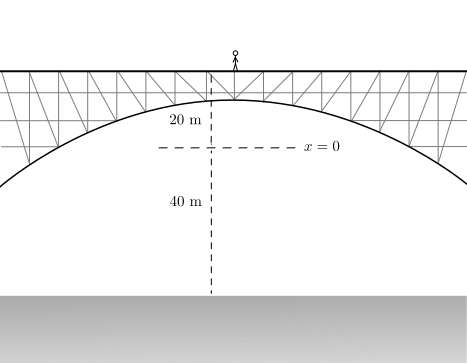
\includegraphics[width=\textwidth]{Bungee_bridge}
\end{figure}




\end{document}
